\subsection{Propuesta de solución}
Se plantea el desarrollo de un prototipo de sistema de monitoreo y control para
la gestión eficiente del consumo de agua en los cultivos de plantas del Vivero
Michita, empleando la metodología de lógica difusa. Este sistema permitirá a
los responsables del vivero supervisar y regular el riego de manera precisa y
adaptativa, optimizando así el uso del recurso hídrico en las áreas de cultivo.
Como se muestra en la Figura \ref{fig:esquema_riego}, el diagrama de procesos
del sistema es fundamental para comprender su estructura. 
\bigbreak 
\bigbreak 
\bigbreak 

\begin{figure}[h]
    \centering
    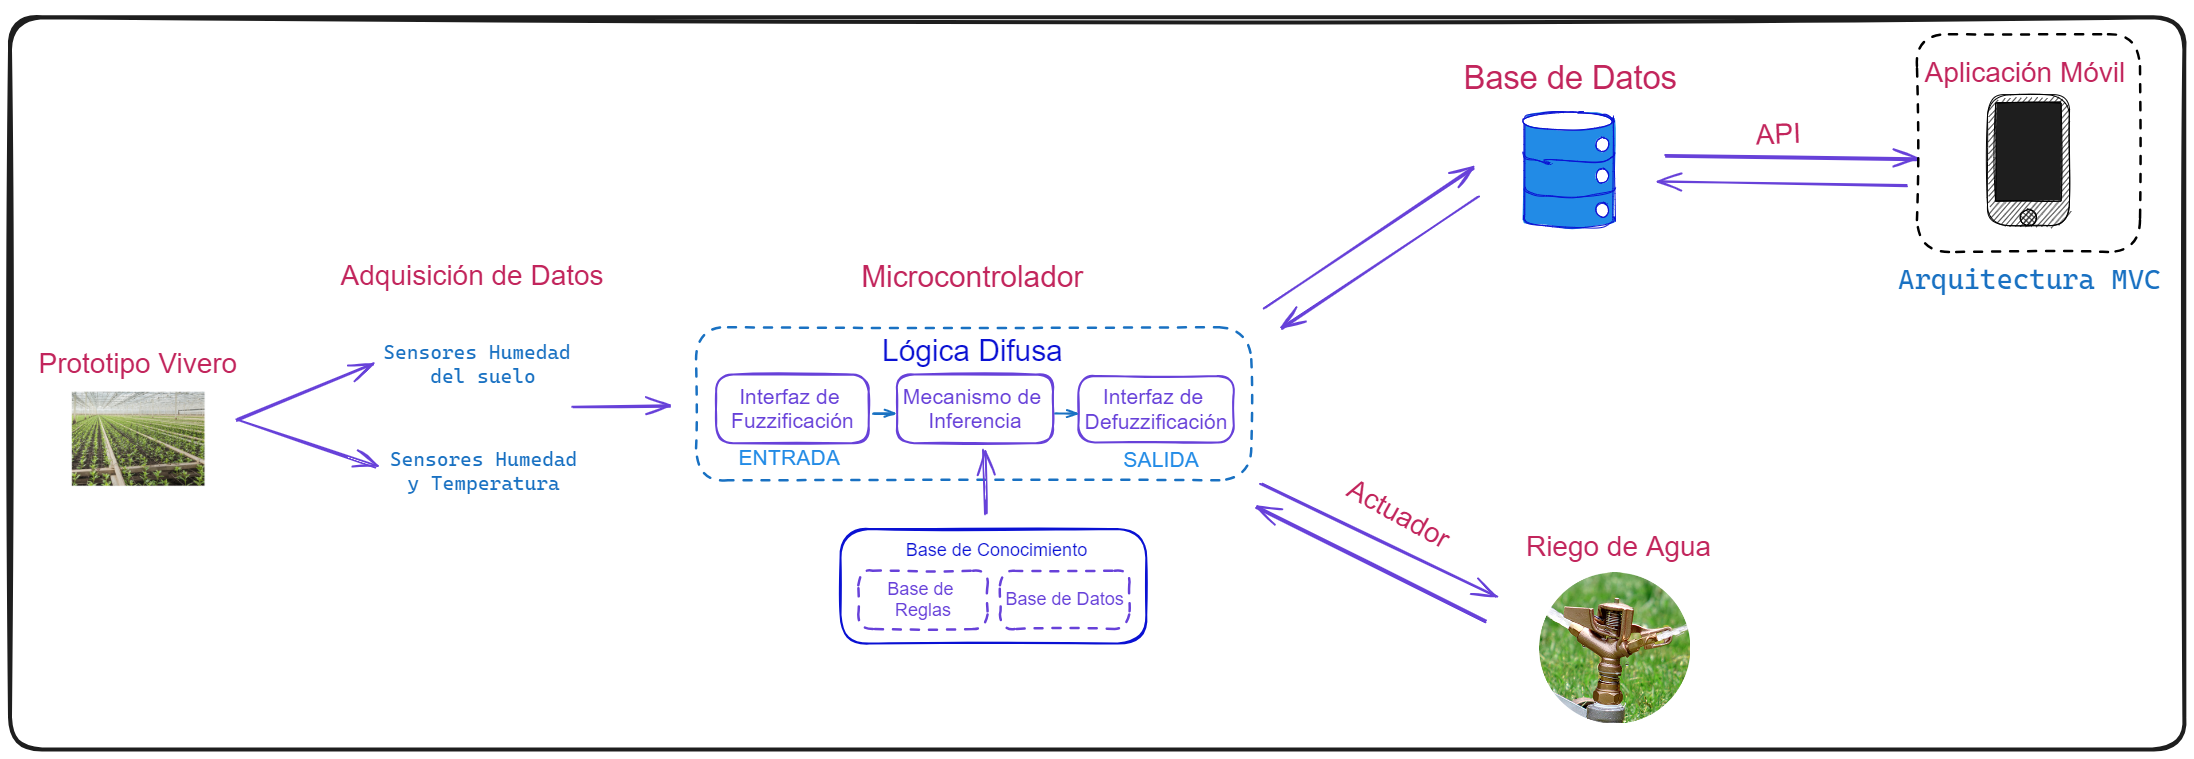
\includegraphics[width=14cm,height=22cm,keepaspectratio]{resources/images/ESQUEMA1.png}
    \caption{Procesos del sistema}
    \label{fig:esquema_riego}
\end{figure}

\begin{itemize}
    \bigbreak 
    \item \textbf{Viabilidad Técnica}
          \bigbreak
          El sistema se diseñará para operar con sensores especializados que monitoreen constantemente la humedad del suelo, las condiciones ambientales y otros parámetros relevantes para determinar las necesidades hídricas de las plantas. Estos datos se procesarán a través de un algoritmo basado en lógica difusa, que tomará decisiones de riego acordes a las condiciones específicas de cada cultivo.

    \item \textbf{Viabilidad Económica}
          \bigbreak
          La implementación de este prototipo posibilitará una gestión más eficiente del riego, permitiendo que los responsables del vivero ajusten el suministro de agua de manera automatizada y precisa. Esto no solo mejorará la salud de las plantas al proporcionarles la cantidad óptima de agua, sino que también optimizará los procesos operativos al reducir la necesidad de supervisiones manuales frecuentes.

    \item \textbf{Viabilidad Operacional}
          \bigbreak
          Desde el punto de vista económico, este prototipo representará una inversión que generará beneficios a largo plazo. La optimización del consumo de agua contribuirá a reducir los costos operativos del vivero, además de disminuir el desperdicio de recursos.
\end{itemize}